% Root file used ashow macros
\documentclass{beamer}
\usepackage{tikz}
\usetikzlibrary{calc}
\usepackage{xcolor}
\usepackage{multicol}
\usepackage{amsmath}
\usepackage{amssymb}

\newcommand{\ablank}[1]{%
  \alt<2>{\textcolor{red}{\underline{#1}}}{\underline{\phantom{#1}}}%
}
\newcommand{\ashow}[1]{\uncover<2->{\textcolor{red}{\small #1}}}
\newcommand{\ashowq}[1]{\alt<2->{\textcolor{red}{\small #1}}{?}}

\title{Percentages: Worked Solutions}
\author{}
\date{}

\begin{document}
\hypersetup{hidelinks}

\frame{\titlepage}

%------------------------------------------------------------------
% CONTENTS
%------------------------------------------------------------------
\begin{frame}[t]{Contents}
\small
\textbf{Questions and short answers}\\
\hyperlink{qslide1}{Starter 1: What is a Percentage?}\\
\hyperlink{qslide2}{Starter 2: Fractions to Percentages}\\
\hyperlink{qslide3}{Starter 3: Converting Fractions to Percentages}\\
\hyperlink{qslide4}{Starter 4: Adding Fractions and Percentages}\\
\hyperlink{qslide5}{Starter 5: Percentages of Amounts}\\
\hyperlink{qslide6}{Starter 6: Percentage Problems}\\
\hyperlink{qslide7}{Starter 7: Decimals to Percentages}\\
\hyperlink{qslide8}{Starter 8: Fractions, Decimals and Percentages}\\
\hyperlink{qslide9}{Starter 9: Review}

\medskip
\textbf{Worked solutions}\\
\hyperlink{wslide1}{Starter 1 worked solutions}\\
\hyperlink{wslide2}{Starter 2 worked solutions}\\
\hyperlink{wslide3}{Starter 3 worked solutions}\\
\hyperlink{wslide4}{Starter 4 worked solutions}\\
\hyperlink{wslide5}{Starter 5 worked solutions}\\
\hyperlink{wslide6}{Starter 6 worked solutions}\\
\hyperlink{wslide7}{Starter 7 worked solutions}\\
\hyperlink{wslide8}{Starter 8 worked solutions}\\
\hyperlink{wslide9}{Starter 9 worked solutions}
\end{frame}

%------------------------------------------------------------------
% QUESTIONS AND SHORT ANSWERS
%------------------------------------------------------------------
\begin{frame}[t,label=qslide1]{Starter 1: What is a Percentage?}
\begin{columns}
\column{0.4\textwidth}
\begin{center}
\vspace{-1.5em}
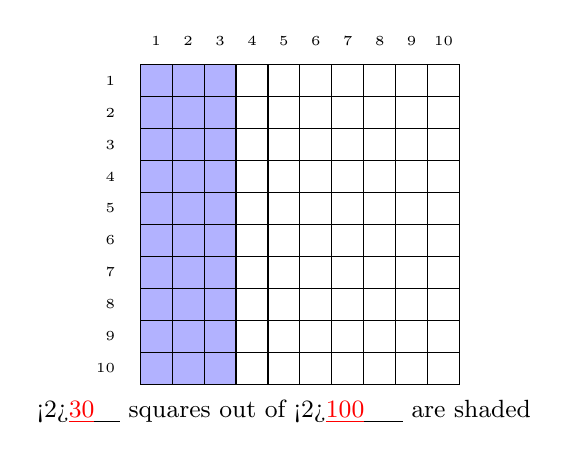
\begin{tikzpicture}[scale=0.78]
\foreach \col in {0,...,9}{
  \foreach \row in {0,...,9}{
    \ifnum\col<3
      \fill[blue!30] (\col*0.52,\row*0.52) rectangle ++(0.52,0.52);
    \fi
    \draw (\col*0.52,\row*0.52) rectangle ++(0.52,0.52);
  }
}
\foreach \col in {0,...,9}{
  \node[font=\tiny, above] at (\col*0.52+0.26, 5.2+0.15) {\number\numexpr\col+1};
}
\foreach \row in {0,...,9}{
  \node[font=\tiny, left] at (-0.25, \row*0.52+0.26) {\number\numexpr10-\row};
}
\node at (2.34,-0.45) {\small \ablank{30} squares out of \ablank{100} are shaded };
\end{tikzpicture}
\end{center}

\column{0.6\textwidth}
\vspace{-1.5em}
\begin{enumerate}
  \item In the diagram how many squares are shaded?
        \ablank{30}
  \item How many total squares are there?
        \ablank{100}
  \item $70 + 30 = \ablank{100}$
  \item $25 \times 4 = \ablank{100}$
  \item What fraction of the square is shaded:
        \ashow{$\tfrac{30}{100}$}
  \item ``Per cent'' means ``out of \ablank{100}''.
  \item The shaded fraction $= \ablank{30\%}$
  \item Write $\dfrac{1}{2}$ as a percentage. \ablank{$50\%$}
  \item Write $\dfrac{1}{4}$ as a percentage. \ablank{$25\%$}
  \item Write $\dfrac{5}{4}$ as a percentage. \ablank{$125\%$}
\end{enumerate}
\end{columns}
\end{frame}

\begin{frame}[t,label=qslide2]{Starter 2: Fractions to Percentages}
\begin{columns}
\column{0.48\textwidth}
\vspace{-4em}
\begin{center}
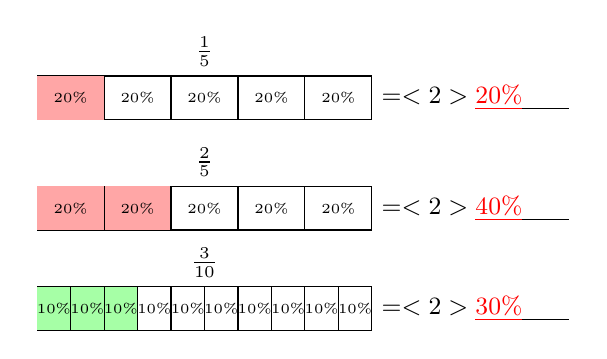
\begin{tikzpicture}[scale=0.85]
\draw (0,0) rectangle (5.0,0.65);
\fill[red!35] (0,0) rectangle (1.0,0.65);
\foreach \x in {1,2,3,4} \draw (\x,0) -- (\x,0.65);
\foreach \i in {0,1,2,3,4}
  \node[font=\tiny] at (\i +0.50,0.325) {20\%};
\node[above,font=\small] at (2.5,0.65) {$\tfrac{1}{5}$};
\node[right,font=\small] at (5.0,0.325) {$=\ablank{20\%}$};

\draw (0,-1.65) rectangle (5.0,-1.0);
\fill[red!35] (0,-1.65) rectangle (2.0,-1.0);
\foreach \x in {1,2,3,4} \draw (\x,-1.65) -- (\x,-1.0);
\foreach \i in {0,1,2,3,4}
  \node[font=\tiny] at (\i+0.50,-1.325) {20\%};
\node[above,font=\small] at (2.5,-1.0) {$\tfrac{2}{5}$};
\node[right,font=\small] at (5.0,-1.325) {$=\ablank{40\%}$};

\draw (0,-3.15) rectangle (5.0,-2.5);
\fill[green!35] (0,-3.15) rectangle (1.50,-2.5);
\foreach \x in {0.50,1.0,...,5.00} \draw (\x,-3.15) -- (\x,-2.5);
\foreach \i in {0,...,9}
  \node[font=\tiny] at (\i*0.50+0.25,-2.825) {10\%};
\node[above,font=\small] at (2.5,-2.5) {$\tfrac{3}{10}$};
\node[right,font=\small] at (5.0,-2.825) {$=\ablank{30\%}$};
\end{tikzpicture}
\end{center}

\column{0.52\textwidth}
\vspace{-2em}
\begin{multicols}{2}
\begin{enumerate}
   \setlength{\itemsep}{12pt}
  \item $3 \times 20 = \ablank{60}$
  \item $7 \times 10 = \ablank{70}$
  \item $\dfrac{1}{5} = \ablank{20\%}$
  \item $\dfrac{2}{5} = \ablank{40\%}$
  \item $\dfrac{3}{10} = \ablank{30\%}$
  \item $\dfrac{\ashowq{7}}{10} = 70\%$
  \item $\dfrac{1}{\ashowq{4}} = 25\%$
  \item $\dfrac{2}{25} = \ablank{8\%}$
  \item $\dfrac{7}{8} = \ablank{87.5\%}$
  \end{enumerate}
\end{multicols}
\begin{center}
  \begin{enumerate}
  \setcounter{enumi}{9}
  \item $\dfrac{5}{3}={}$\ablank{$166.\dot{6}\%$}
  \vspace{0.6em}
  \item Complete the conversion: \\[2pt]
        $\dfrac{\ashowq{3}}{4} = \dfrac{75}{\ashowq{100}} = 75\%$
\end{enumerate}
\end{center}
\end{columns}
\end{frame}

\begin{frame}[t,label=qslide3]{Starter 3: Converting Fractions to Percentages}
\begin{columns}
\column{0.35\textwidth}
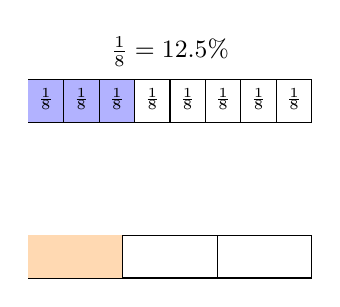
\begin{tikzpicture}[scale=0.9]
\draw (0,0) rectangle (4,0.6);
\fill[blue!30] (0,0) rectangle (1.5,0.6);
\foreach \x in {0.5,1.0,1.5,2.0,2.5,3.0,3.5}
  \draw (\x,0) -- (\x,0.6);
\foreach \i in {0.5,1.0,1.5,2.0,2.5,3.0,3.5,4.0}
  \node[font=\tiny] at (\i-0.25,0.325) {$\frac{1}{8}$};
\node[above,font=\small] at (2,0.65) {$\frac{1}{8} = 12.5\%$};
\draw (0,-2.2) rectangle (4,-1.6);
\fill[orange!30] (0,-2.2) rectangle (1.333,-1.6);
\draw (1.333,-2.2) -- (1.333,-1.6);
\draw (2.667,-2.2) -- (2.667,-1.6);
\end{tikzpicture}

\column{0.65\textwidth}
\textbf{Questions}
\begin{enumerate}
  \item Write $\frac{1}{2}$ as a percentage. \ablank{$50\%$}
  \item Write $\frac{3}{10}$ as a percentage. \ablank{$30\%$}
  \item What does ``per cent'' mean? \ablank{out of 100}
  \item Convert $\frac{3}{8}$ to a percentage. \ablank{$37.5\%$}
  \item What percentage of the second bar is shaded orange? \ablank{$33.\dot{3}\%$}
  \item Convert $\frac{2}{3}$ to a percentage. \ablank{$66.\dot{6}\%$}
  \item What is $\frac{4}{3}$ as a percentage, round your percentage to one decimal place. \ablank{$133.3\%$}
  \item What fraction does $0.1\%$ equal? \ashow{$\frac{1}{1000}$}
  \item What fraction does $0.003\%$ equal? \ashow{$\frac{3}{100,000}$}
\end{enumerate}
\end{columns}
\end{frame}

\begin{frame}[t,label=qslide4]{Starter 4: Adding Fractions and Percentages}
\begin{columns}
\column{0.35\textwidth}
\begin{center}
\vspace{-5em}
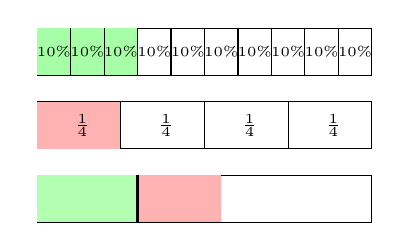
\begin{tikzpicture}[scale=0.85]
\draw (0,0) rectangle (5.0,0.7);
\fill[green!35] (0,0) rectangle (1.50,0.7);
\foreach \x in {0.50,1.0,...,5.00} \draw (\x,0) -- (\x,0.7);
\foreach \i in {0,...,9}
  \node[font=\tiny] at (\i*0.50+0.25,0.35) {10\%};

\draw (0,-1.1) rectangle (5,-0.4);
\fill[red!30] (0,-1.1) rectangle (1.25,-0.4);
\foreach \x in {1.25,2.5,3.75} \draw (\x,-1.1) -- (\x,-0.4);
\foreach \i in {0,...,3}
    \node[font=\tiny] at (\i*1.25+0.675,-0.75) {$\frac{1}{4}$};

\draw (0,-2.2) rectangle (5,-1.5);
\fill[green!30] (0,-2.2) rectangle (1.5,-1.5);
\fill[red!30] (1.5,-2.2) rectangle (2.75,-1.5);
\draw[thick] (1.5,-2.2) -- (1.5,-1.5);
\end{tikzpicture}
\end{center}

\column{0.7\textwidth}
\vspace{-2em}
\begin{enumerate}
\begin{multicols}{2}
  \item $50\% + 50\% = \ablank{100\%}$
  \item $25\% + 25\% = \ablank{50\%}$
\end{multicols}
  \item Write $\frac{1}{5}$ as a percentage: \ablank{$20\%$}
  \item Complete the sum represented by the diagram: \\[0.2em]
  $ 3 \times \ashowq{10}\% + \frac{1}{\ashowq{4}} = 30\% + 25\% = 55\% $
\begin{multicols}{2}
  \item $20\%+\dfrac{3}{10}=\ablank{50\%}$
  \item $\dfrac{1}{2}+15\%=\ablank{65\%}$
  \item $45\%+\dfrac{1}{5}=\ablank{65\%}$
  \item Which is larger: $\dfrac{3}{8}$ or $40\%$?
        \ablank{$40\%$ ($\tfrac{3}{8}=37.5\%$)}
  \item $\dfrac{2}{5}+\dfrac{3}{10}+20\%=\ablank{90\%}$
\end{multicols}

  \item A class finishes $\tfrac{1}{3}$ of a project, then $20\%$ more. What percentage have they completed in total?
        \ashow{$33.\dot{3}\%+20\%=53.\dot{3}\%$}
\end{enumerate}
\end{columns}
\end{frame}

\begin{frame}[t,label=qslide5]{Starter 5: Percentages of Amounts}
\begin{columns}
\column{0.40\textwidth}
\begin{center}
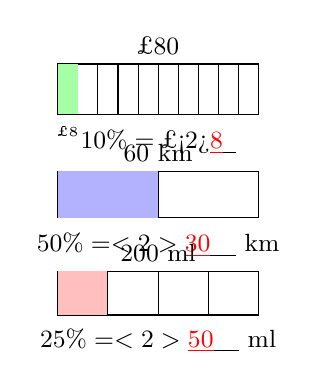
\begin{tikzpicture}[scale=0.85]
\draw (0,0) rectangle (3,0.75);
\foreach \x in {0.3,0.6,...,2.9} \draw (\x,0) -- (\x,0.75);
\fill[green!35] (0,0) rectangle (0.3,0.75);
\node[above,font=\small] at (1.5,0.75) {\pounds 80};
\node[below,font=\tiny] at (0.15,-0.05) {\pounds 8};
\node[font=\small] at (1.5,-0.42) {$10\%={}$\pounds\ablank{8}};
\draw (0,-1.55) rectangle (3,-0.85);
\fill[blue!30] (0,-1.55) rectangle (1.5,-0.85);
\draw (1.5,-1.55) -- (1.5,-0.85);
\node[above,font=\small] at (1.5,-0.85) {60 km};
\node[font=\small] at (1.5,-1.95) {$50\%=\ablank{30}$ km};
\draw (0,-3.0) rectangle (3,-2.35);
\fill[red!25] (0,-3.0) rectangle (0.75,-2.35);
\foreach \x in {0.75,1.5,2.25} \draw (\x,-3.0) -- (\x,-2.35);
\node[above,font=\small] at (1.5,-2.35) {200 ml};
\node[font=\small] at (1.5,-3.38) {$25\%=\ablank{50}$ ml};
\end{tikzpicture}
\end{center}

\column{0.60\textwidth}
\textbf{Find the percentage of the amount:}
\begin{enumerate}
  \item $10\%$ of \pounds90 $={}$\pounds\ablank{9}
  \item $50\%$ of \pounds46 $={}$\pounds\ablank{23}
  \item $25\%$ of $200=\ablank{50}$
  \item $30\%$ of \pounds50 $={}$\pounds\ablank{15}
  \item $15\%$ of \pounds80 $={}$\pounds\ablank{12}
  \item Jacket: \pounds120, reduced by $35\%$. Saving?
        \ashow{$0.35\times120=\pounds42$}
  \item $17.5\%$ of \pounds240 $={}$\pounds\ablank{42}
  \item \textit{Challenge:} 840 pupils; $62.5\%$ go on trip.
        How many stay?
        \ashow{$525$ go; $840-525=315$ stay.}
\end{enumerate}
\end{columns}
\end{frame}

\begin{frame}[t,label=qslide6]{Starter 6: Percentage Problems}
\begin{columns}
\column{0.40\textwidth}
\begin{center}
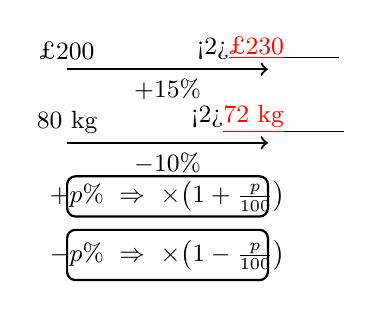
\begin{tikzpicture}[scale=0.85]
\draw[thick,->] (0,0.3) -- (3,0.3);
\node[above,font=\small] at (0,0.3) {\pounds 200};
\node[above,font=\small] at (3,0.3) {\ablank{\pounds 230}};
\node[below,font=\small] at (1.5,0.3) {$+15\%$};
\draw[thick,->] (0,-0.8) -- (3,-0.8);
\node[above,font=\small] at (0,-0.8) {80 kg};
\node[above,font=\small] at (3,-0.8) {\ablank{72 kg}};
\node[below,font=\small] at (1.5,-0.8) {$-10\%$};
\draw[rounded corners=3pt,thick] (0,-1.9) rectangle (3,-1.3);
\node[font=\small] at (1.5,-1.6) {$+p\%\ \Rightarrow\ \times\!\left(1+\tfrac{p}{100}\right)$};
\draw[rounded corners=3pt,thick] (0,-2.85) rectangle (3,-2.1);
\node[font=\small] at (1.5,-2.48) {$-p\%\ \Rightarrow\ \times\!\left(1-\tfrac{p}{100}\right)$};
\end{tikzpicture}
\end{center}

\column{0.60\textwidth}
\textbf{Questions}
\begin{enumerate}
  \item Increase \pounds60 by $20\%$: \ablank{\pounds72}
  \item Decrease 150 by $40\%$: \ablank{90}
  \item Phone: \pounds350, reduced $12\%$. New price?
        \ashow{$350\times0.88=\pounds308$}
  \item $60\%$ of 300 students study French.
        How many? \ablank{180}
  \item Salary \pounds28\,000 rises $5\%$. New salary?
        \ashow{$28000\times1.05=\pounds29\,400$}
  \item VAT at $20\%$ added to \pounds45. Total?
        \ablank{\pounds54}
  \item \textit{Challenge:} TV reduced $15\%$ to \pounds340.
        Original price?
        \ashow{$340\div0.85=\pounds400$}
\end{enumerate}
\end{columns}
\end{frame}

\begin{frame}[t,label=qslide7]{Starter 7: Decimals to Percentages}
\begin{columns}
\column{0.4\textwidth}
\begin{center}
\vspace{-1em}
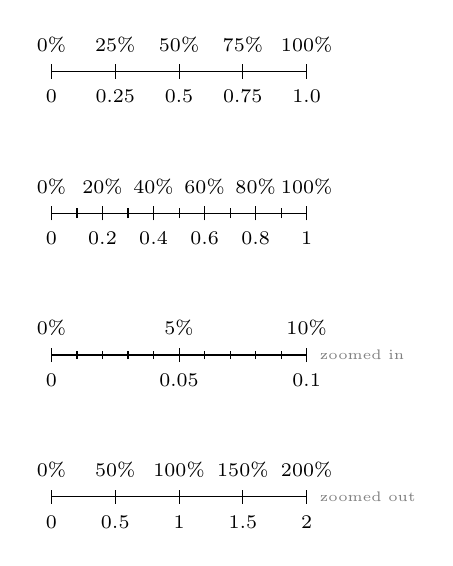
\begin{tikzpicture}[scale=0.9, every node/.style={font=\scriptsize}]

\def\Y{0}
\def\W{3.6}
\draw (0,\Y) -- (\W,\Y);
\foreach \frac/\dec/\pct in {%
    0/{0}/{0\%}, 1/{0.25}/{25\%}, 2/{0.5}/{50\%},
    3/{0.75}/{75\%}, 4/{1.0}/{100\%}}{
  \pgfmathsetmacro\xx{\frac*\W/4}
  \draw (\xx,\Y-0.10) -- (\xx,\Y+0.10);
  \node[below] at (\xx,\Y-0.13) {\dec};
  \node[above] at (\xx,\Y+0.13) {\pct};
}

\def\Y{-2.0}
\draw (0,\Y) -- (\W,\Y);
\foreach \k in {0,1,...,10}{
  \pgfmathsetmacro\xx{\k*\W/10}
  \pgfmathsetmacro\dec{\k/10}
  \ifodd\k
    \draw (\xx,\Y-0.07) -- (\xx,\Y+0.07);
  \else
    \draw (\xx,\Y-0.10) -- (\xx,\Y+0.10);
    \node[below] at (\xx,\Y-0.13) {\pgfmathprintnumber[fixed,precision=1]{\dec}};
    \pgfmathsetmacro\pct{int(\k*10)}
    \node[above] at (\xx,\Y+0.13) {\pct\%};
  \fi
}
\pgfmathsetmacro\ta{0.92*\W}

\def\Y{-4.0}
\draw (0,\Y) -- (\W,\Y);
\foreach \k/\dec/\pct in {0/{0}/{0\%}, 1/{0.05}/{5\%}, 2/{0.1}/{10\%}}{
  \pgfmathsetmacro\xx{\k*\W/2}
  \draw (\xx,\Y-0.10) -- (\xx,\Y+0.10);
  \node[below] at (\xx,\Y-0.13) {\dec};
  \node[above] at (\xx,\Y+0.13) {\pct};
}
\foreach \k in {1,2,...,9}{
  \pgfmathsetmacro\xx{\k*\W/10}
  \draw (\xx,\Y-0.06) -- (\xx,\Y+0.06);
}
\node[right,gray] at (\W+0.05,\Y) {\tiny zoomed in};

\def\Y{-6.0}
\draw (0,\Y) -- (\W,\Y);
\foreach \k in {0,1,2,3,4}{
  \pgfmathsetmacro\xx{\k*\W/4}
  \pgfmathsetmacro\dec{\k/2}
  \pgfmathsetmacro\pct{int(\k*50)}
  \draw (\xx,\Y-0.10) -- (\xx,\Y+0.10);
  \node[below] at (\xx,\Y-0.13) {\pgfmathprintnumber[fixed,precision=1]{\dec}};
  \node[above] at (\xx,\Y+0.13) {\pct\%};
}
\node[right,gray] at (\W+0.05,\Y) {\tiny zoomed out};
\end{tikzpicture}
\end{center}

\column{0.60\textwidth}
\begin{enumerate}
\begin{multicols}{2}
  \item $0.6 + 0.4 = \ablank{1}$
  \item $0.25 \times 4 = \ablank{1}$
\end{multicols}
  \item Write $\frac{3}{10}$ as a decimal: \ablank{$0.3$}
  \item Write $\frac{7}{100}$ as a decimal: \ablank{$0.07$}
\begin{multicols}{2}
  \item $0.5   = \ablank{50\%}$
  \item $0.3   = \ablank{30\%}$
  \item $0.75  = \ablank{75\%}$
  \item $0.08  = \ablank{8\%}$
  \item $0.125 = \ablank{12.5\%}$
  \item $1.4   = \ablank{140\%}$
  \item $0.005 = \ablank{0.5\%}$
  \item $0.92  \to \ablank{92\%}$
\end{multicols}
  \item \textit{Challenge:} Convert $0.0625$ to a \%,\\
        then write as a fraction in simplest form.
        \ashow{$6.25\%=\tfrac{1}{16}$}
\end{enumerate}
\end{columns}
\end{frame}

\begin{frame}[t,label=qslide8]{Starter 8: Fractions, Decimals and Percentages}
\vspace{-2em}
\begin{columns}

\column{0.38\textwidth}
\begin{center}
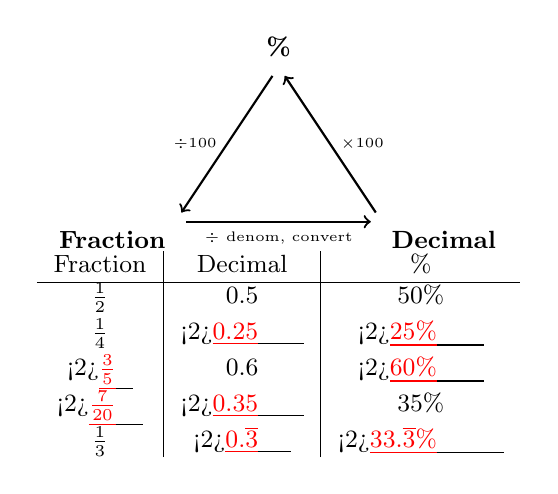
\begin{tikzpicture}[scale=0.82]
\coordinate (F) at (0,0);
\coordinate (D) at (3.2,0);
\coordinate (P) at (1.6,2.4);
\draw[->,thick,shorten >=4pt,shorten <=4pt] (F) -- node[below,font=\tiny]{$\div$ denom, convert} (D);
\draw[->,thick,shorten >=4pt,shorten <=4pt] (D) -- node[right,font=\tiny]{$\times100$} (P);
\draw[->,thick,shorten >=4pt,shorten <=4pt] (P) -- node[left,font=\tiny]{$\div100$} (F);
\node[below left,font=\small] at (F) {\textbf{Fraction}};
\node[below right,font=\small] at (D) {\textbf{Decimal}};
\node[above,font=\small] at (P) {\textbf{\%}};
\node at (1.6,-2.05) {\small
\begin{tabular}{c|c|c}
Fraction & Decimal & \% \\ \hline
$\tfrac{1}{2}$ & $0.5$ & $50\%$ \\[2pt]
$\tfrac{1}{4}$ & \ablank{0.25} & \ablank{25\%} \\[2pt]
\ablank{$\tfrac{3}{5}$} & $0.6$ & \ablank{60\%} \\[2pt]
\ablank{$\tfrac{7}{20}$} & \ablank{0.35} & $35\%$ \\[2pt]
$\tfrac{1}{3}$ & \ablank{$0.\overline{3}$} & \ablank{$33.\overline{3}\%$}
\end{tabular}};
\end{tikzpicture}
\end{center}

\column{0.62\textwidth}
\small
\begin{multicols}{2}
\begin{enumerate}
  \item $0.45=\ablank{45}\%$
  \item $72\%$ as decimal: \ablank{0.72}
  \item $\dfrac{9}{20}$ as \%: \ablank{45\%}
  \item $0.375$ as fraction: \ablank{$\tfrac{3}{8}$}
  \item Order smallest to largest:\\
        $0.6,\ \tfrac{5}{9},\ 58\%$\\
        \ashow{$\tfrac{5}{9}{\approx}55.6\%{<}58\%{<}60\%$}

  \columnbreak

  \item $130\%$ as decimal: \ablank{1.3}
  \item $1.05$ as \%: \ablank{105\%}
  \item Which is largest?
        \vspace{-4pt}
        \[ \tfrac{7}{12},\quad 0.59,\quad 57\% \]
        \vspace{-10pt}
        \ashow{$\tfrac{7}{12}{\approx}58.3\%$ largest}
  \item \textit{Challenge:} Order\\
        $\tfrac{7}{9},\ 0.7\overline{8},\ 78.5\%$\\
        \ashow{$\approx77.8\%{<}78.5\%{<}78.9\%$}
\end{enumerate}
\end{multicols}
\end{columns}
\end{frame}

\begin{frame}[t,label=qslide9]{Starter 9: Review}
\vspace{-2.5em}
\begin{columns}

\column{0.28\textwidth}
\begin{center}
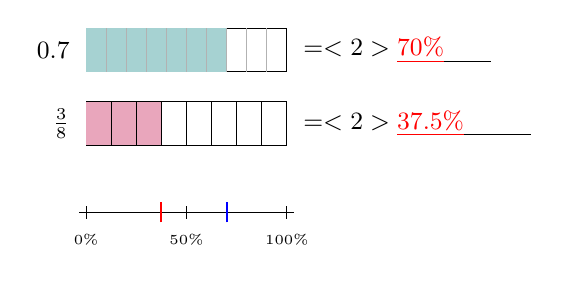
\begin{tikzpicture}[scale=0.85]
\draw (0,0) rectangle (3,0.65);
\fill[teal!35] (0,0) rectangle (2.1,0.65);
\foreach \x in {0.3,0.6,...,2.9} \draw[gray!60] (\x,0) -- (\x,0.65);
\node[left,font=\small] at (-0.1,0.325) {$0.7$};
\node[right,font=\small] at (3.1,0.325) {$=\ablank{70\%}$};
\draw (0,-1.1) rectangle (3,-0.45);
\fill[purple!35] (0,-1.1) rectangle (1.125,-0.45);
\foreach \x in {0.375,0.75,1.125,1.5,1.875,2.25,2.625}
  \draw (\x,-1.1) -- (\x,-0.45);
\node[left,font=\small] at (-0.1,-0.775) {$\tfrac{3}{8}$};
\node[right,font=\small] at (3.1,-0.775) {$=\ablank{37.5\%}$};
\draw (-0.1,-2.1) -- (3.1,-2.1);
\foreach \x/\lab in {0/{$0\%$},1.5/{$50\%$},3/{$100\%$}}{
  \draw (\x,-2.2) -- (\x,-2.0);
  \node[below,font=\tiny] at (\x,-2.28) {\lab};
}
\draw[red,thick] (1.125,-2.25) -- (1.125,-1.95);
\draw[blue,thick] (2.1,-2.25) -- (2.1,-1.95);
\end{tikzpicture}
\end{center}

\column{0.72\textwidth}
\small
\begin{multicols}{2}
\begin{enumerate}
  \item $\dfrac{3}{4}=\ablank{75}\%$
  \item $0.06=\ablank{6}\%$
  \item $\dfrac{5}{8}=\ablank{62.5}\%$
  \item $110\%$ as decimal: \ablank{1.1}
  \item $35\%$ of \pounds60 $={}$\pounds\ablank{21}
  \item Increase \pounds80 by $15\%$: \ablank{\pounds92}

  \columnbreak

  \item Decrease 240 by $12.5\%$: \ablank{210}
  \item $\dfrac{2}{3}+15\%={}$\ablank{$81.\overline{6}\%$}
  \item Order: $0.7,\ \tfrac{3}{4},\ 72\%$\\
        \ashow{$70\%<72\%<75\%$}
  \item \textit{Challenge:} Item: $-20\%$, then $-10\%$ more. Same as $-30\%$?\\
        \ashow{$\times0.8\times0.9{=}\times0.72$. That's $28\%$ off, not $30\%$!}
\end{enumerate}
\end{multicols}
\end{columns}
\end{frame}

%------------------------------------------------------------------
% WORKED SOLUTIONS
%------------------------------------------------------------------
\begin{frame}[t,label=wslide1]{Starter 1, Question 1}
\textbf{Working:} The shaded region is 3 full columns. Each column contains 10 squares, so the number of shaded squares is \(3\times 10\).
\par\medskip
\textbf{Answer:} \ashow{$30$}
\end{frame}

\begin{frame}[t]{Starter 1, Question 2}
\textbf{Working:} The grid is \(10\) squares wide and \(10\) squares high, so the total number of squares is \(10\times 10\).
\par\medskip
\textbf{Answer:} \ashow{$100$}
\end{frame}

\begin{frame}[t]{Starter 1, Question 3}
\textbf{Working:} \(70\) is 7 tens and \(30\) is 3 tens. Together they make 10 tens, which is \(10\times 10\).
\par\medskip
\textbf{Answer:} \ashow{$100$}
\end{frame}

\begin{frame}[t]{Starter 1, Question 4}
\textbf{Working:} Think of \(25\) as one quarter of \(100\), so four quarters make the whole.
\par\medskip
\textbf{Answer:} \ashow{$100$}
\end{frame}

\begin{frame}[t]{Starter 1, Question 5}
\textbf{Working:} The fraction shaded is the number of shaded squares divided by the total number of squares. There are 30 shaded squares out of 100 total.
\par\medskip
\textbf{Answer:} \ashow{$\tfrac{30}{100}$}
\end{frame}

\begin{frame}[t]{Starter 1, Question 6}
\textbf{Working:} The word ``per cent'' comes from the Latin \emph{per centum}, meaning ``by the hundred''.
\par\medskip
\textbf{Answer:} \ashow{out of 100}
\end{frame}

\begin{frame}[t]{Starter 1, Question 7}
\textbf{Working:} Since the shaded fraction is \(\frac{30}{100}\), write this as \(30\) out of \(100\).
\par\medskip
\textbf{Answer:} \ashow{$30\%$}
\end{frame}

\begin{frame}[t]{Starter 1, Question 8}
\textbf{Working:} Multiply numerator and denominator by 50:
\[
\frac{1}{2}=\frac{50}{100}.
\]
\par\medskip
\textbf{Answer:} \ashow{$50\%$}
\end{frame}

\begin{frame}[t]{Starter 1, Question 9}
\textbf{Working:} Multiply numerator and denominator by 25:
\[
\frac{1}{4}=\frac{25}{100}.
\]
\par\medskip
\textbf{Answer:} \ashow{$25\%$}
\end{frame}

\begin{frame}[t]{Starter 1, Question 10}
\textbf{Working:} \(\frac54=5\times\frac14\), and \(\frac14=25\%\), so \(\frac54=5\times25\%\).
\par\medskip
\textbf{Answer:} \ashow{$125\%$}
\end{frame}

\begin{frame}[t,label=wslide2]{Starter 2, Question 1}
\textbf{Working:} \(3\times 20 = 3\times 2\times 10 = 6\times 10\).
\par\medskip
\textbf{Answer:} \ashow{$60$}
\end{frame}

\begin{frame}[t]{Starter 2, Question 2}
\textbf{Working:} \(7\times 10=70\).
\par\medskip
\textbf{Answer:} \ashow{$70$}
\end{frame}

\begin{frame}[t]{Starter 2, Question 3}
\textbf{Working:} \(\frac15\) is equivalent to \(\frac{20}{100}\).
\par\medskip
\textbf{Answer:} \ashow{$20\%$}
\end{frame}

\begin{frame}[t]{Starter 2, Question 4}
\textbf{Working:} \(\frac25\) is equivalent to \(\frac{40}{100}\).
\par\medskip
\textbf{Answer:} \ashow{$40\%$}
\end{frame}

\begin{frame}[t]{Starter 2, Question 5}
\textbf{Working:} \(\frac{3}{10}\) is equivalent to \(\frac{30}{100}\).
\par\medskip
\textbf{Answer:} \ashow{$30\%$}
\end{frame}

\begin{frame}[t]{Starter 2, Question 6}
\textbf{Working:} \(70\%=\frac{70}{100}\). Divide numerator and denominator by 10:
\[
\frac{70}{100}=\frac{7}{10}.
\]
\par\medskip
\textbf{Answer:} \ashow{$7$}
\end{frame}

\begin{frame}[t]{Starter 2, Question 7}
\textbf{Working:} \(25\%=\frac{25}{100}\). Divide numerator and denominator by 25:
\[
\frac{25}{100}=\frac14.
\]
\par\medskip
\textbf{Answer:} \ashow{$4$}
\end{frame}

\begin{frame}[t]{Starter 2, Question 8}
\textbf{Working:} \(25\times 4=100\), so multiply numerator and denominator by 4:
\[
\frac{2}{25}=\frac{8}{100}.
\]
\par\medskip
\textbf{Answer:} \ashow{$8\%$}
\end{frame}

\begin{frame}[t]{Starter 2, Question 9}
\textbf{Working:} \(\frac18=12.5\%\), so \(\frac78=7\times 12.5\%\).
\par\medskip
\textbf{Answer:} \ashow{$87.5\%$}
\end{frame}

\begin{frame}[t]{Starter 2, Question 10}
\textbf{Working:} \(\frac53=1.666\ldots\), so as a percentage it is \(166.666\ldots\%\).
\par\medskip
\textbf{Answer:} \ashow{$166.\dot{6}\%$}
\end{frame}

\begin{frame}[t]{Starter 2, Question 11}
\textbf{Working:} \(75\%=\frac{75}{100}\). Divide numerator and denominator by 25:
\[
\frac{75}{100}=\frac34.
\]
So the missing numerator is 3 and the missing denominator is 100.
\par\medskip
\textbf{Answer:} \ashow{$3$} and \ashow{$100$}
\end{frame}

\begin{frame}[t,label=wslide3]{Starter 3, Question 1}
\textbf{Working:} \(\frac12=0.5=50\%\).
\par\medskip
\textbf{Answer:} \ashow{$50\%$}
\end{frame}

\begin{frame}[t]{Starter 3, Question 2}
\textbf{Working:} \(\frac{3}{10}=\frac{30}{100}\).
\par\medskip
\textbf{Answer:} \ashow{$30\%$}
\end{frame}

\begin{frame}[t]{Starter 3, Question 3}
\textbf{Working:} ``Per cent'' means ``by the hundred'' or ``out of 100''.
\par\medskip
\textbf{Answer:} \ashow{out of 100}
\end{frame}

\begin{frame}[t]{Starter 3, Question 4}
\textbf{Working:} \(\frac18=12.5\%\), so \(\frac38=3\times 12.5\%\).
\par\medskip
\textbf{Answer:} \ashow{$37.5\%$}
\end{frame}

\begin{frame}[t]{Starter 3, Question 5}
\textbf{Working:} The second bar is split into 3 equal pieces and one piece is shaded, so the shaded fraction is \(\frac13\).
\par\medskip
\textbf{Answer:} \ashow{$33.\dot{3}\%$}
\end{frame}

\begin{frame}[t]{Starter 3, Question 6}
\textbf{Working:} \(\frac13=33.\dot3\%\), so \(\frac23=2\times 33.\dot3\%\).
\par\medskip
\textbf{Answer:} \ashow{$66.\dot{6}\%$}
\end{frame}

\begin{frame}[t]{Starter 3, Question 7}
\textbf{Working:} \(\frac43=1.333\ldots\), so as a percentage it is \(133.333\ldots\%\). Rounded to 1 decimal place:
\par\medskip
\textbf{Answer:} \ashow{$133.3\%$}
\end{frame}

\begin{frame}[t]{Starter 3, Question 8}
\textbf{Working:} \(0.1\%=\frac{0.1}{100}=\frac{1}{1000}\).
\par\medskip
\textbf{Answer:} \ashow{$\frac{1}{1000}$}
\end{frame}

\begin{frame}[t]{Starter 3, Question 9}
\textbf{Working:} \(0.003\%=\frac{0.003}{100}=\frac{3}{100000}\).
\par\medskip
\textbf{Answer:} \ashow{$\frac{3}{100{,}000}$}
\end{frame}

\begin{frame}[t,label=wslide4]{Starter 4, Question 1}
\textbf{Working:} \(50\%+50\%=100\%\).
\par\medskip
\textbf{Answer:} \ashow{$100\%$}
\end{frame}

\begin{frame}[t]{Starter 4, Question 2}
\textbf{Working:} \(25\%+25\%=50\%\).
\par\medskip
\textbf{Answer:} \ashow{$50\%$}
\end{frame}

\begin{frame}[t]{Starter 4, Question 3}
\textbf{Working:} \(\frac15=\frac{20}{100}\).
\par\medskip
\textbf{Answer:} \ashow{$20\%$}
\end{frame}

\begin{frame}[t]{Starter 4, Question 4}
\textbf{Working:} The diagram shows three 10\% blocks and one quarter. Three blocks give \(30\%\), and \(\frac14=25\%\). Together they give \(30\%+25\%\).
\par\medskip
\textbf{Answer:} \ashow{$10$} and \ashow{$4$}
\end{frame}

\begin{frame}[t]{Starter 4, Question 5}
\textbf{Working:} \(\frac{3}{10}=30\%\), so \(20\%+\frac{3}{10}=20\%+30\%\).
\par\medskip
\textbf{Answer:} \ashow{$50\%$}
\end{frame}

\begin{frame}[t]{Starter 4, Question 6}
\textbf{Working:} \(\frac12=50\%\), so \(\frac12+15\%=50\%+15\%\).
\par\medskip
\textbf{Answer:} \ashow{$65\%$}
\end{frame}

\begin{frame}[t]{Starter 4, Question 7}
\textbf{Working:} \(\frac15=20\%\), so \(45\%+\frac15=45\%+20\%\).
\par\medskip
\textbf{Answer:} \ashow{$65\%$}
\end{frame}

\begin{frame}[t]{Starter 4, Question 8}
\textbf{Working:} \(\frac38=37.5\%\), which is less than \(40\%\).
\par\medskip
\textbf{Answer:} \ashow{$40\%$}
\end{frame}

\begin{frame}[t]{Starter 4, Question 9}
\textbf{Working:} Convert everything to percentages:
\[
\frac25=40\%,\quad \frac{3}{10}=30\%,\quad 20\%.
\]
Now add: \(40\%+30\%+20\%\).
\par\medskip
\textbf{Answer:} \ashow{$90\%$}
\end{frame}

\begin{frame}[t]{Starter 4, Question 10}
\textbf{Working:} \(\frac13=33.\dot3\%\). Then add the extra \(20\%\):
\[
33.\dot3\%+20\%.
\]
\par\medskip
\textbf{Answer:} \ashow{$53.\dot{3}\%$}
\end{frame}

\begin{frame}[t,label=wslide5]{Starter 5, Question 1}
\textbf{Working:} \(10\%=\frac{1}{10}\), so \(10\%\) of \(\pounds 90\) is \(90\div 10\).
\par\medskip
\textbf{Answer:} \ashow{\pounds 9}
\end{frame}

\begin{frame}[t]{Starter 5, Question 2}
\textbf{Working:} \(50\%=\frac12\), so \(50\%\) of \(\pounds46\) is \(46\div2\).
\par\medskip
\textbf{Answer:} \ashow{\pounds 23}
\end{frame}

\begin{frame}[t]{Starter 5, Question 3}
\textbf{Working:} \(25\%=\frac14\), so \(25\%\) of \(200\) is \(200\div4\).
\par\medskip
\textbf{Answer:} \ashow{$50$}
\end{frame}

\begin{frame}[t]{Starter 5, Question 4}
\textbf{Working:} \(10\%\) of \(\pounds50\) is \(\pounds5\), so \(30\%\) is \(3\times\pounds5\).
\par\medskip
\textbf{Answer:} \ashow{\pounds 15}
\end{frame}

\begin{frame}[t]{Starter 5, Question 5}
\textbf{Working:} \(10\%\) of \(\pounds80\) is \(\pounds8\), and \(5\%\) is \(\pounds4\). So \(15\%\) is \(\pounds8+\pounds4\).
\par\medskip
\textbf{Answer:} \ashow{\pounds 12}
\end{frame}

\begin{frame}[t]{Starter 5, Question 6}
\textbf{Working:} The saving is \(35\%\) of \(\pounds120\).
\[
0.35\times 120=42.
\]
\par\medskip
\textbf{Answer:} \ashow{\pounds 42}
\end{frame}

\begin{frame}[t]{Starter 5, Question 7}
\textbf{Working:} Use \(17.5\%=10\%+5\%+2.5\%\).
\[
10\%\text{ of }240=24,\quad 5\%=12,\quad 2.5\%=6.
\]
So \(24+12+6=42\).
\par\medskip
\textbf{Answer:} \ashow{\pounds 42}
\end{frame}

\begin{frame}[t]{Starter 5, Question 8}
\textbf{Working:} \(62.5\%=\frac58\). The number who stay is:
\[
840-\frac58\times840.
\]
\par\medskip
\textbf{Answer:} \ashow{315}
\end{frame}

\begin{frame}[t,label=wslide6]{Starter 6, Question 1}
\textbf{Working:} Increasing by \(20\%\) means multiplying by \(1.20\).
\[
60\times1.20=72.
\]
\par\medskip
\textbf{Answer:} \ashow{\pounds 72}
\end{frame}

\begin{frame}[t]{Starter 6, Question 2}
\textbf{Working:} Decreasing by \(40\%\) means multiplying by \(0.60\).
\[
150\times0.60=90.
\]
\par\medskip
\textbf{Answer:} \ashow{90}
\end{frame}

\begin{frame}[t]{Starter 6, Question 3}
\textbf{Working:} Reducing by \(12\%\) means multiplying by \(0.88\).
\[
350\times0.88=308.
\]
\par\medskip
\textbf{Answer:} \ashow{\pounds 308}
\end{frame}

\begin{frame}[t]{Starter 6, Question 4}
\textbf{Working:} \(60\%=0.60\), so \(0.60\times300\).
\par\medskip
\textbf{Answer:} \ashow{180}
\end{frame}

\begin{frame}[t]{Starter 6, Question 5}
\textbf{Working:} A \(5\%\) rise means multiplying by \(1.05\).
\[
28000\times1.05=29400.
\]
\par\medskip
\textbf{Answer:} \ashow{\pounds 29\,400}
\end{frame}

\begin{frame}[t]{Starter 6, Question 6}
\textbf{Working:} Adding \(20\%\) VAT means multiplying by \(1.20\).
\[
45\times1.20=54.
\]
\par\medskip
\textbf{Answer:} \ashow{\pounds 54}
\end{frame}

\begin{frame}[t]{Starter 6, Question 7}
\textbf{Working:} If the price was reduced by \(15\%\), the sale price is \(85\%\) of the original, so multiply by \(0.85\). Thus original price is \(340\div0.85\).
\par\medskip
\textbf{Answer:} \ashow{\pounds 400}
\end{frame}

\begin{frame}[t,label=wslide7]{Starter 7, Question 1}
\textbf{Working:} \(0.6+0.4\) is 6 tenths plus 4 tenths, which is 10 tenths.
\par\medskip
\textbf{Answer:} \ashow{$1$}
\end{frame}

\begin{frame}[t]{Starter 7, Question 2}
\textbf{Working:} \(0.25=\frac14\), and \(4\times\frac14=1\).
\par\medskip
\textbf{Answer:} \ashow{$1$}
\end{frame}

\begin{frame}[t]{Starter 7, Question 3}
\textbf{Working:} \(\frac{3}{10}\) means 3 tenths.
\par\medskip
\textbf{Answer:} \ashow{$0.3$}
\end{frame}

\begin{frame}[t]{Starter 7, Question 4}
\textbf{Working:} \(\frac{7}{100}\) means 7 hundredths.
\par\medskip
\textbf{Answer:} \ashow{$0.07$}
\end{frame}

\begin{frame}[t]{Starter 7, Question 5}
\textbf{Working:} Multiply \(0.5\) by 100 to get a percentage: \(0.5\times100=50\).
\par\medskip
\textbf{Answer:} \ashow{$50\%$}
\end{frame}

\begin{frame}[t]{Starter 7, Question 6}
\textbf{Working:} \(0.3\times100=30\).
\par\medskip
\textbf{Answer:} \ashow{$30\%$}
\end{frame}

\begin{frame}[t]{Starter 7, Question 7}
\textbf{Working:} \(0.75\times100=75\).
\par\medskip
\textbf{Answer:} \ashow{$75\%$}
\end{frame}

\begin{frame}[t]{Starter 7, Question 8}
\textbf{Working:} \(0.08\times100=8\).
\par\medskip
\textbf{Answer:} \ashow{$8\%$}
\end{frame}

\begin{frame}[t]{Starter 7, Question 9}
\textbf{Working:} \(0.125=\frac{125}{1000}=\frac{12.5}{100}\).
\par\medskip
\textbf{Answer:} \ashow{$12.5\%$}
\end{frame}

\begin{frame}[t]{Starter 7, Question 10}
\textbf{Working:} \(1.4=1+0.4\). Since \(1=100\%\) and \(0.4=40\%\), the total is \(100\%+40\%\).
\par\medskip
\textbf{Answer:} \ashow{$140\%$}
\end{frame}

\begin{frame}[t]{Starter 7, Question 11}
\textbf{Working:} \(0.005=\frac{5}{1000}=\frac{0.5}{100}\).
\par\medskip
\textbf{Answer:} \ashow{$0.5\%$}
\end{frame}

\begin{frame}[t]{Starter 7, Question 12}
\textbf{Working:} \(0.92\times100=92\).
\par\medskip
\textbf{Answer:} \ashow{$92\%$}
\end{frame}

\begin{frame}[t]{Starter 7, Question 13}
\textbf{Working:} \(0.0625\times100=6.25\), so \(0.0625=6.25\%\).
As a fraction,
\[
6.25\%=\frac{6.25}{100}=\frac{625}{10000}=\frac{1}{16}.
\]
\par\medskip
\textbf{Answer:} \ashow{$6.25\%=\tfrac{1}{16}$}
\end{frame}

\begin{frame}[t,label=wslide8]{Starter 8, Question 1}
\textbf{Working:} Multiply \(0.45\) by 100.
\par\medskip
\textbf{Answer:} \ashow{$45\%$}
\end{frame}

\begin{frame}[t]{Starter 8, Question 2}
\textbf{Working:} Divide \(72\) by 100: \(72\%=\frac{72}{100}\).
\par\medskip
\textbf{Answer:} \ashow{$0.72$}
\end{frame}

\begin{frame}[t]{Starter 8, Question 3}
\textbf{Working:} \(\frac{9}{20}=\frac{45}{100}\).
\par\medskip
\textbf{Answer:} \ashow{$45\%$}
\end{frame}

\begin{frame}[t]{Starter 8, Question 4}
\textbf{Working:} \(0.375=\frac{375}{1000}\). Divide numerator and denominator by 125:
\[
\frac{375}{1000}=\frac38.
\]
\par\medskip
\textbf{Answer:} \ashow{$\tfrac{3}{8}$}
\end{frame}

\begin{frame}[t]{Starter 8, Question 5}
\textbf{Working:} Convert to percentages:
\[
\frac59\approx55.6\%,\quad 58\%,\quad 0.6=60\%.
\]
\par\medskip
\textbf{Answer:} \ashow{$\tfrac{5}{9}<58\%<0.6$}
\end{frame}

\begin{frame}[t]{Starter 8, Question 6}
\textbf{Working:} \(130\%=\frac{130}{100}\).
\par\medskip
\textbf{Answer:} \ashow{$1.3$}
\end{frame}

\begin{frame}[t]{Starter 8, Question 7}
\textbf{Working:} \(1.05\times100=105\).
\par\medskip
\textbf{Answer:} \ashow{$105\%$}
\end{frame}

\begin{frame}[t]{Starter 8, Question 8}
\textbf{Working:} Convert to percentages:
\[
\frac{7}{12}\approx58.3\%,\quad 57\%.
\]
Since \(0.59=59\%\), \(0.59\) is larger than \(58.3\%\).
\par\medskip
\textbf{Answer:} \ashow{$0.59$}
\end{frame}

\begin{frame}[t]{Starter 8, Question 9}
\textbf{Working:} Convert to decimals or percentages:
\[
\frac79\approx0.777\ldots\approx77.8\%,\quad
0.7\overline{8}\approx78.9\%,\quad 78.5\%.
\]
\par\medskip
\textbf{Answer:} \ashow{$\tfrac{7}{9}<78.5\%<0.7\overline{8}$}
\end{frame}

\begin{frame}[t,label=wslide9]{Starter 9, Question 1}
\textbf{Working:} \(\frac34=\frac{75}{100}\).
\par\medskip
\textbf{Answer:} \ashow{$75\%$}
\end{frame}

\begin{frame}[t]{Starter 9, Question 2}
\textbf{Working:} \(0.06\times100=6\).
\par\medskip
\textbf{Answer:} \ashow{$6\%$}
\end{frame}

\begin{frame}[t]{Starter 9, Question 3}
\textbf{Working:} \(\frac18=12.5\%\), so \(\frac58=5\times12.5\%\).
\par\medskip
\textbf{Answer:} \ashow{$62.5\%$}
\end{frame}

\begin{frame}[t]{Starter 9, Question 4}
\textbf{Working:} \(110\%=\frac{110}{100}\).
\par\medskip
\textbf{Answer:} \ashow{$1.1$}
\end{frame}

\begin{frame}[t]{Starter 9, Question 5}
\textbf{Working:} \(10\%\) of \(\pounds60\) is \(\pounds6\), so \(30\%\) is \(\pounds18\) and \(5\%\) is \(\pounds3\).
\[
18+3=21.
\]
\par\medskip
\textbf{Answer:} \ashow{\pounds 21}
\end{frame}

\begin{frame}[t]{Starter 9, Question 6}
\textbf{Working:} Increasing by \(15\%\) means multiplying by \(1.15\).
\[
80\times1.15=92.
\]
\par\medskip
\textbf{Answer:} \ashow{\pounds 92}
\end{frame}

\begin{frame}[t]{Starter 9, Question 7}
\textbf{Working:} \(12.5\%=\frac18\). So the decrease is \(240\div8=30\), and the new amount is \(240-30\).
\par\medskip
\textbf{Answer:} \ashow{210}
\end{frame}

\begin{frame}[t]{Starter 9, Question 8}
\textbf{Working:} \(\frac23=66.\dot6\%\). Add \(15\%\):
\[
66.\dot6\%+15\%=81.\dot6\%.
\]
\par\medskip
\textbf{Answer:} \ashow{$81.\overline{6}\%$}
\end{frame}

\begin{frame}[t]{Starter 9, Question 9}
\textbf{Working:} Convert to percentages:
\[
0.7=70\%,\quad \frac34=75\%,\quad 72\%.
\]
\par\medskip
\textbf{Answer:} \ashow{$0.7<72\%<\tfrac{3}{4}$}
\end{frame}

\begin{frame}[t]{Starter 9, Question 10}
\textbf{Working:} A decrease of \(20\%\) gives multiplier \(0.8\). Another decrease of \(10\%\) gives multiplier \(0.9\).
\[
0.8\times0.9=0.72.
\]
This means the final price is \(72\%\) of the original, so the total decrease is \(28\%\), not \(30\%\).
\par\medskip
\textbf{Answer:} \ashow{No, \(28\%\) off, not \(30\%\)}
\end{frame}

\end{document}